\section{Technology Stack}

The feature hypothesis (\autoref{sub:hypothesis}) states that networking,
persistence, serialization, session management and game engine integration are
necessary to build a fully functional \og{}. These essential features are
mandatory to drive an \og{}.

In addition to these core technologies, supplementary technologies are needed to
help fulfill the deployment and the simple development hypothesis
(\autoref{sub:hypothesis}). These technologies are: container engine,
composition engine, continuous integration solution, source control system, and
\glsreset{ide}\gls{ide}.

The rest of this section describes each technology and states advantages and
disadvantages along with the arguments which are decisive for the composition
of the technology stack.

\subsection{Core Technologies}

The core technologies have mostly been defined and tested in the prior two
project theses. This section only gives a short summary on the chosen
technologies.

\subsubsection{Networking}

\begin{wrapfigure}{r}{4cm}
	\vspace*{-0.2cm}
    
\includegraphics[width=4cm]{images/dependencies/activemq}
\end{wrapfigure}

\textbf{ActiveMQ} is a popular message broker. A message broker buffers
messages and delivers them as soon as a receiver is available. This allows for a
robust and persistent messaging. Message brokers have been evaluated during
project thesis one. ActiveMQ is the networking foundation of MicroNet and
has proven to be very stable. ActiveMQ is supplied with a Java JMS library which
provides a way to easily integrate ActiveMQ into Java applications.

ActiveMQ is available on Docker Hub as a Docker image and can therefore easily
be integrated into a \ms{} application using a composition engine.


\subsubsection{Persistence and Session Management}

\begin{wrapfigure}{r}{4cm}
 	\hspace*{0.4cm}
    
\includegraphics[width=4cm]{images/dependencies/PostgreSQL}
\end{wrapfigure}

\textbf{PostgreSQL} is a very mature open source relational database. It is
available on all major platforms, which allows for comfortable testing and
deployment. Since version 9.2 PostgreSQL supports the \gls{json} data-type,
which makes it trivial to control the data flow from the network to the database.

PostgreSQL is also available on Docker hub and can therefore be quickly
integrated. For production purposes a native installation of PostgreSQL is
suggested to provide the needed stability as explained in
\autoref{sub:database_solutions}.\\ 


\begin{wrapfigure}{r}{4cm}
    
\includegraphics[width=4cm]{images/dependencies/couchbase}
\end{wrapfigure}

\noindent \textbf{Couchbase} is a NoSQL database realized as a \gls{json}
document store. The \gls{json} affinity of Couchbase cooperates very well with
the technology stack. Couchbase has its own query language called N1QL which
allows aggregated queries between multiple documents. Also access on
sub-document level is possible to allow fine grained data access.

Couchbase can run in a cluster and maintains a quorum on each document to
provide eventual consistency on document write operations. The cluster
functionality can be used to scale the database system. Couchbase also provides
timeouts of documents which can be used to imitate \textit{session store}
behaviour to facilitate session management. This neglects the need for a
distributed caching system like Redis.

Even if Couchbase exists as a Docker image it is advised for production to
install a native version of Coutchbase for the reasons explained in
\autoref{sub:database_solutions}. For testing the containerized version can be
very helpful due to the quick setup. This is further supported by the fact that
Couchbase is schema-less which further simplifies the installation process. 
    
\newpage
\subsubsection{Serialization}

\begin{wrapfigure}{r}{4cm}
    
\includegraphics[width=4cm]{images/dependencies/google-gson}
\end{wrapfigure}

\textbf{Gson} from Google offers a very convenient out-of-the-box approach to
serialize Java objects to \gls{json} strings and vice versa. It is an additional
advantage of Gson to supports generic collections like hash-maps.

The main advantage of Gson is its simplicity. The simplicity happens at the
expense of of performance especially for the de-serialization of \gls{json}
Strings. Because of this reason simple Gson serialization is only useful in
areas where a performance hit does not influence the application behaviour.

\subsubsection{Game Engine Integration}

\begin{wrapfigure}{r}{4cm}
    
\includegraphics[width=4cm]{images/dependencies/Unity3D}
\end{wrapfigure}
    
\textbf{Unity3D} is very popular among independent developers because it has no
initial financial barrier. Unity3D is very well documented and has a very
healthy community to provide support for development problems.

Unity3D provides a rich editor that may be used to prototype games quickly. It
also offers a rich C\# \gls{api} which is used to write any imaginable game
simulation logic.

For this thesis it is of particular interest to see how well the combination of
C\# game logic and Java back-end logic works in regard to the \ms{} tenet of
polyglot programming.
    
\subsection{Supplementary Technologies}

The supplementary technologies have been under intense evaluation during the
process of this thesis. The result of this evaluation is a set of augmenting
technologies which work well together, are easy to learn, and are open source or
have a community edition (free of charge and maintained by the community).

\subsubsection{Container Engine}

\begin{wrapfigure}{r}{4cm}
	\vspace*{-0.5cm} \hspace*{0.2cm}
    
\includegraphics[width=3cm]{images/dependencies/docker}
\end{wrapfigure}

\textbf{Docker} has already been mentioned several times in this document.
The essence about Docker is that it is an enabler technology. This is because
all other composition and container technologies support Docker in some way.
This aspect makes Docker Engine a reliable intermediate layer between the actual
hardware and the application running on it.

\newpage
\subsubsection{Composition Engine}

\begin{wrapfigure}{r}{4cm}
	\vspace*{-0.5cm} \hspace*{0.8cm}
    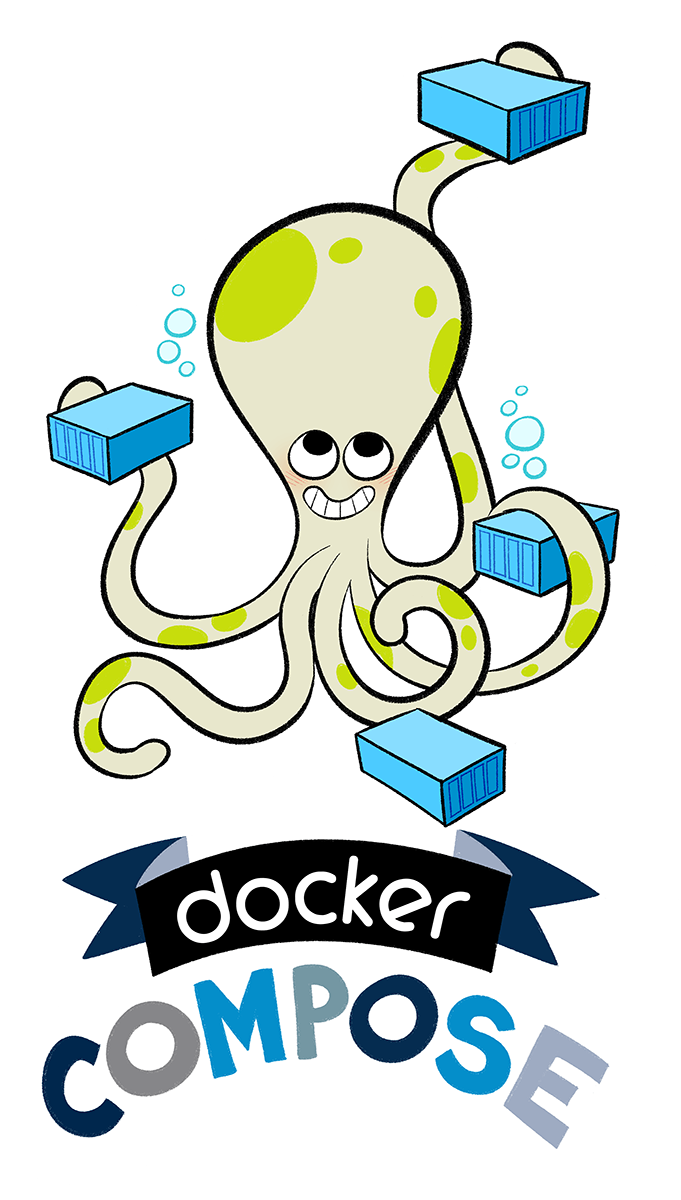
\includegraphics[width=2.4cm]{images/dependencies/docker-compose}
\end{wrapfigure}

\textbf{Docker-compose} is basically only a CLI application which translates a
docker-compose file into a set of docker commands which are sequentially
executed. The result is a containerized application running on a single
host. Docker-compose is very helpful to quickly deploy a \ms{} application
stack locally. The docker-compose format also provides the basis to deploy a
composed application in the cloud using docker-swarm.\\

\begin{wrapfigure}{r}{4cm}
	\hspace*{0.4cm}
    
\includegraphics[width=3.3cm]{images/dependencies/docker-swarm}
\end{wrapfigure}

\noindent\textbf{Docker-swarm} is used to run containerized applications on a
cluster of Docker machines. A Docker machine is simply a host running a Docker
engine. Docker swarm allows to deploy each services of an application
individually using the docker stack CLI and also offers the possibility to
deploy a complete application stack defined through a docker-compose file.
Docker swarm offers multiple scheduling strategies which distribute the
containers among the available docker machines.

The major advantage of Docker swarm is its simplicity. Only a few commands are
needed to control the cluster so docker-swarm is therefore easy to understand.
Since it is the native Docker composition technology it is also a natural match
for containerized Docker applications.

One noticeable disadvantage is the lack of several convenience features like a
build-in dashboard or auto-scaling support. This is not a big concern since many
third party dashboard tools like Grafana are available and auto-scaling can be
added with a little bit of an implementation effort.

\subsubsection{Continuous Integration}

Continuous integration is generally a part of every software project and \ogs{}
are no exception. In this thesis the continuous integration process is examined
up to the point where all individual steps of the process are defined. From here
a central build system like Jenkins can take over and unify the whole build
process, but this aspect is not covered in this thesis.\\

\begin{wrapfigure}{r}{4cm}
    
\includegraphics[width=4cm]{images/dependencies/maven}
\end{wrapfigure}

\noindent\textbf{Maven} is a build system and provides a convenient way to
define the build process of Java applications. For the game back-end services
which are mainly written in Java this is a perfect match to define the build
process.

Maven also works very well in cooperation with Docker. A dedicated Maven Docker
image can be used to easily integrate the Java build process into the Docker
build process by executing the Maven build inside the target container. This approach
removes the need of any local Java or Maven installation. 

The drawback of the complete in-container Maven build is its performance.
Maven downloads ``the whole Internet'' into every container to build the
application. This is not useful during development where short build times are
mandatory. In order to cope with this problem the Maven build can be conducted
on the host system and only the binaries (executable Jars in case of Java
services) are sent to the Docker daemon for the container build process. This
makes the combined build process much faster and has no real disadvantage
because the process can be exactly reproduced on the build system and therefore
also speeds up automated builds.

Maven is also very useful to preserve a consistent versioning of \mss{}. The
game application stack can be described using a master .pom file containing
the required versions of all services. The master .pom file can be updated to
introduce a new version of any service. The continuous integration process can
be triggered at this point to perform a rolling update of the currently
deployed application stack.\\
	


\subsubsection{Source Control System}

A source control system is mandatory in every software project to keep track of
artifacts and versions. Source control is important to safely store the source
code of an application but also to provide source level access to many open
source projects like MicroNet.\\

\begin{wrapfigure}{r}{4cm}
    
\includegraphics[width=4cm]{images/dependencies/github}
\end{wrapfigure}

\textbf{Git} is the \textit{Source Control System} that builds the foundation
for the version control. Git works perfectly to share Maven projects which in
turn is used to reproduce the build process locally and also on a build server.

Github is used to provide any needed dependency used for the build process.
MicroNet is also published via Github.

\subsubsection{Interactive Development Environment (IDE)}

\gls{ide} is a wide term for a tool that simplifies the development process of a
software program. Usually it provides comprehensive tools that assist in writing
the source code of an application.\\

\begin{wrapfigure}{r}{4cm}
    
\includegraphics[width=4cm]{images/dependencies/eclipse}
\end{wrapfigure}

\noindent\textbf{Eclipse provides} a very solid \gls{ide} to develop Java
projects. The plug-in development environment of Eclipse can be used to
customize the \gls{ide} to an arbitrary extent. This aspect is especially useful
because almost no specific \ms{} development tools are available on the market.
Also Eclipse provides a number of very useful plug-ins for Java development.

The \textit{Docker Tools} for Eclipse consist of a visual explorer for Docker
images and containers. It allows to quickly start, stop, build and remove containers
without having to bother with console commands.

\textit{Launch Groups} is a plug-in contributed by Eclipse CDT (C++ development
plug-in for Eclipse). It is very useful to directly run or debug multiple
applications at once. This allows to quickly bring up or terminate the whole
application stack for testing purposes. Although CDT is required for Launch
Groups it does not interfere with Java development.































